\documentclass{article}

\PassOptionsToPackage{numbers, compress}{natbib}
\usepackage[final]{nips_2017}
\usepackage{listings}
\usepackage{textcomp}
\usepackage[usenames,dvipsnames,svgnames]{xcolor}
\usepackage{graphicx}
\usepackage[subrefformat=parens]{subcaption}
\usepackage{amssymb}

\newcommand{\expr}[0]{\texttt{<expr>}}
\newcommand{\address}[0]{\texttt{<address>}}
\newcommand{\genaddr}[0]{\mathtt{@addr}}
\newcommand{\genbackprop}[0]{\mathtt{backprop}}
\newcommand{\gentracegrad}[0]{\mathtt{trace\_gradient}}
\newcommand{\gengen}[0]{\mathtt{@gen}}
\newcommand{\code}[1]{\mbox{\texttt{#1}}}

%!TEX root = ./main.tex

\lstset{
  basicstyle=\ttfamily\scriptsize,
  columns=fullflexible,
  keepspaces=true,
  upquote=true,
  % Define . and % and @ as letters to include them in keywords.
  alsoletter={\.,\%,\#, \@, \?, \/},
  % First type of keywords.
  morekeywords=[1]{function, if, else, end, for, begin, in, const, struct, using, return},
  keywordstyle=[1]\textcolor{Brown},
  % Second type of keywords.
  morekeywords=[2]{\@gen, \@rand, \@param, \@input, \@output, \@tf_function, \@call, \@read, \@tf_call},
  keywordstyle=[2]\textcolor{RoyalBlue},
  % Add strings
  showstringspaces=False,
  %stringstyle=\ttfamily\color{NavyBlue},
  %stringstyle=\ttfamily\color{Purple},
  %morestring=[b]{"},
  %morestring=[b]{'},
  % l is for line comment
  morecomment=[l]{\#},
  commentstyle=\color{Gray}\ttfamily,
  escapeinside={<@}{@>}
}

\newcommand{\addr}[1]{\textcolor{DarkGreen}{#1}}


\title{Probabilistic programming with programmable deep learning and Monte Carlo inference in GenLite}

\author{
  Marco F.~Cusumano-Towner\thanks{MIT Probabilistic Computing Project and Computer Science and Artificial Intelligence Laboratory}\\
  Massachusetts Institute of Technology\\
  \texttt{marcoct@mit.edu} \\
  \And
  Vikash K.~Mansinghka\thanks{MIT Probabilistic Computing Project and Department of Brain and Cognitive Sciences}\\
  Massachusetts Institute of Technology\\
  \texttt{vkm@mit.edu}
}


\begin{document}

\maketitle
\setcounter{footnote}{0}

\begin{abstract}
Probabilistic programming provides concise and flexible languages for generative modeling, but achieving reliably efficient inference in probabilistic programming systems based on automated Monte Carlo algorithms remains challenging.
Recently, user-programmable inference and offline training of proposal distributions based on deep neural networks have been proposed as two solutions to this problem.
This paper proposes to combine these two approaches by permitting users to define parametrized proposal distributions as probabilistic programs based on deep neural networks.
Users train these networks on data simulated from the generative model, which is also represented as a probabilistic program.
The paper demonstrates the approach with models and inference programs written in GenLite, a probabilistic programming language with user-programmable inference that uses TensorFlow for scalable deep learning.
\end{abstract}

\section{Introduction}

\section{Probabilistic programming with custom inference in GenLite}

\subsection{Generative functions}

\subsubsection{Random choices}

\subsubsection{Reading from an input trace}

\subsubsection{Trainable static parameters}

\subsubsection{Calling other generative functions}

\subsection{Selection functions}

\subsection{High-level embedded inference programming}

\subsubsection{Traces are user-space Julia values}

\subsubsection{Observation traces}

\subsubsection{Monte Carlo inference operators}

% imp, imp2, mh, mh2

% the full set of inference operators, and the semantics of these operators, are outside the scope of this paper

\subsubsection{Training generative functions using $\genbackprop{}$}

\subsubsection{Gradient-based MAP using $\gentracegrad{}$}

GenLite \cite{TODO} is a flexible probabilistic programming language designed to support user-programmable inference.
This section provides a very brief introduction to GenLite.
GenLite is embedded in Julia \cite{TODO}.
In GenLite, users first express a probabilistic generative model as a \emph{generative function}, which is written in an embedded DSL that extends Julia functions with the ability to make traced random choies.
Then, users implement Monte Carlo inference algorithms for the model in Julia code, drawing heavily on GenLite's inference programming API, which provides core data structures and inference primitives that utilize the programmatic representation of the generative model.
User inference code is written at a higher level of abstraction than typical custom sampler implementations, which makes it more efficient to develop, maintain, and reason about.

In GenLite, a \emph{trace} is a Julia value (of type \texttt{Trace}) that contains a record of random choices made by some generative function.
Generative functions, which are declared with keyword \texttt{@gen function}, extend Julia with four language constructs:
\begin{enumerate}
\item \texttt{@rand(<expr>, <address>)}: Sample a random value (i.e. a `random choice') from probability distribution \expr{}, where \address{} is a string or tuple of strings that specify a hierarchical name, or `address' for the random choice.
Record the random choice in the trace at the given address.
\item \texttt{@call(<expr>, <address>)}: Invoke a generative function given by \expr{}, and record the resulting trace for the invoked function under address \address{} in the current trace.
\item \texttt{@read(<address>)}: If an input trace is provided, read the value in the input trace at the given \address{}.
This feature is used by generative functions that represent proposal distributions (see below).
\item \texttt{@param <name>::<type>}: Declare a trainable parameter of a generative function, which is static (i.e. the same value is shared by all invocations of the generative function).
Static parameters are initialized by the user outside of the generative function body.
\end{enumerate}

Note that generative functions can contain arbitrary Julia code.
Figure~\ref{fig:model-code-figure} shows a generative function that only exercises the \texttt{@rand} keyword.
In addition to generative models, proposal distributions for MCMC and importance sampling can also be expressed as generative functions \cite{cusumano2018using}.

The GenLite inference programming API contains a number of methods that implement building blocks for inference and learning algorithms.
A building block that is used for training the static parameters of generative functions is \texttt{backprop}, which has the following type signature:
\begin{center}
    \texttt{backprop(fn::GenerativeFunction, args::Tuple, trace::Trace, [input\_trace::Trace])}
\end{center}
The trace must be a complete trace of the given generative function for the given arguments to the function.
This method computes the gradient of the log probability of the trace with respect to all static parameters, using reverse-mode automatic differentiation (AD).
Each static parameter has a \emph{gradient accumulator}, which is a value that is incremented by the gradient during each call to \texttt{backprop}.
User Julia code reads and write to the gradient accumulator values and the values of static parameters to perform parameter updates, using GenLite methods:\\
\texttt{set\_param!(fn::GenerativeFunction, name::Symbol, value)}\\
\texttt{get\_param(fn::GenerativeFunction, name::Symbol)}\\
\texttt{get\_param\_grad(fn::GenerativeFunction, name::Symbol)}\\
\texttt{zero\_param\_grad!(fn::GenerativeFunction, name::Symbol)}


\section{Training Custom Proposals on Simulated Data}

% math relating KL and maximum likelihood

As shown in \cite{cusumano2018using}, proposals represented as generative functions for MCMC and importance sampling can be trained on data simulated from a model to improve the efficiency of the Monte Carlo algorithm.
A similar approach was proposed by \cite{le2016inference} for use in training a general-purpose neural network for inference in probabilistic programs.
We briefly summarize the key mathematical ideas here.
Let $x$ and $y$ denote the values of latent variables and observable variables respectively (e.g. in the model of Figure~\ref{fig:model-code-figure}, the latent variables are the parameters of the glyph, and the observable variable is the noisy image).
Let $p(x, y)$ denote the joint probability distribution of a generative model for which we want to perform inference about $x$ given $y$, and let $p(y)$ and $p(x)$ denote the two marginal distributions.
We will take a sampling approach to inference.
That is, given some $y$, we seek to sample $x$ with probability $p(x | y) := p(x, y) / p(y)$.
We will assume we have access to a trainable family of proposal distributions denoted $q(x; y, \theta)$.
This is a family of probability distributions on $x$, parametrized by $y$ and $\theta$, where $\theta$ are trainable parameters.
We will train the proposal by approximately solving the following optimization problem:
\[
\min_{\theta} \mathbb{E}_{y \sim p(\cdot)} \left[ \mbox{KL}(p(x | y) || q(x; y, \theta)) \right]
\]
Intuitively, we seek to find a proposal that is close to $p(x | y)$ in KL divergence from $p$ to $q$ for typical observations $y$ sampled from the model's prior distribution on observations ($y \sim p(\cdot)$).
This is equivalent to maximizing the expected conditional log likelihood:
\[
\max_{\theta} \mathbb{E}_{x, y \sim p(\cdot, \cdot)} \left[ \log q(x; y, \theta) \right]
\]
Therefore, we can use stochastic gradient ascent, where we obtain training instances by sampling $x, y \sim p(\cdot, \cdot)$, which amounts to a joint sample from the generative model.
If the generative model is expressed as generative function in GenLite, we can obtain a trace that contains both $x$ and $y$, using the \texttt{simulate} API method:
\begin{center}
    \texttt{(trace::Trace, score, val) = simulate(::GenerativeFunction, args::Tuple)}
\end{center}
If the proposal is also expressed as a generative function, then we can implement $\theta$ using static parameters of the generative function, and compute the required gradients $\nabla_{\theta} \log q(x; y, \theta)$ using \texttt{backprop}, passing the simulated model trace as both the input trace (from which $y$ will be read) and the trace of the proposal generative function itself (from which $x$ is read).

Once we have a trained proposal, we can use it in a variety of model-based Monte Carlo algorithms, which are able to asymptotically correct for errors in the distribution $q(x; y, \theta)$ relative to the target distribution $p(x | y)$.
For example, if the proposal distribution is typically `too wide' relative to the posterior (which is expected due to the specific direction of KL divergence being optimized), then applying importance sampling with the given proposal is one way of generating asymptotically exact samples from the posterior.
The number of importance samples required to reach a given level of error for some observations $y$ is roughly exponential in the KL divergence $\mbox{KL}(p(x | y) || q(x; y, \theta))$, as shown in recent theoretical work on importance sampling \cite{chatterjee2018sample}.

Note that the same approach can also be used to learn other conditional distributions besides the posterior $p(x | y)$.
For example, if there are two groups of latent variables $x_1$ and $x_2$, we can train two different proposals to match $p(x_1 | x_2, y)$ and $p(x_2 | x_1, y)$, respectively.
These proposals can then be used to approximate a Gibbs sampler.
Finally, note that proposals that generate latent variables given the observations are often called `data-driven proposals' (e.g. \cite{tu2002image}).



\section{Scalable Deep Learning with TensorFlow Integration}

% language (functional subset of TensorFlow with @param)

% implementation (hybrid AD)

Although it is possible to implement deep neural networks in Julia and invoke these from generative functions using static parameters to store network weights, support for GPU and deep learning in Julia is still new.
Therefore, GenLite includes the option of using TensorFlow for deep learning.
We extend GenLite with a \texttt{tf\_function} and \texttt{tf\_call} language constructs.
The \texttt{tf\_function} keyword is used to define \emph{GenLite TensorFlow functions}, which are functional TensorFlow computations with declared inputs, trainable parameters, and an output, that can be invoked by generative functions (see Figure~\ref{fig:proposal-code-figure} for an example).
Within \texttt{tf\_function} blocks, we construct TensorFlow computations using the TensorFlow.jl \cite{?} wrapper around the TensorFlow C API, as well as three new keywords that facilitate integration with GenLite:
\begin{enumerate}
\item \texttt{@input <name> <dtype> <shape>}:
Assigns a TF placeholder with given data type and shape to variable \texttt{name}, and registers this with GenLite as an input of the TF function.
\item \texttt{@param <name> <initial-julia-value>}:
Declare a static parameter for the TensorFlow function.
Assigns a TF variable with given initial value variable \texttt{name}, and registers this with GenLite as an input of the TF function.
GenLite constructs an additional variable to store the accumulated gradient of output with respect to the variable \texttt{<name>}.
\item \texttt{@output <dtype> <tensor-value>}:
Registers the given tensor value as the output of the TF function and statically declares its data type.
\end{enumerate}
Note that static parameters of TensorFlow functions have similar semantics to static parameters of generative functions, but are implemented differently (e.g. the values are owned by the TensorFlow runtime instead of Julia) and are accessed and modified using a different interface (a TensorFlow interface as opposed to a Julia interface).

TensorFlow functions are invoked by generative functions using:
\begin{center}
    \texttt{@tf\_call(<tf-function>([input1, [input2, ..]]))}
\end{center}
where each input is a Julia value corresponding to an \texttt{@input} declaration (in the order of the declarations in the body of the function).
Evaluating a \texttt{@tf\_call} expression invokes the TF computation and returns the tensor registered as \texttt{@output} as a Julia \texttt{Array} value.
When the expression is evaluated in GenLite's \texttt{backprop} API method, evaluating the \texttt{@tf\_call} expression also causes a cell for the TF function to be placed on the GenLite's AD tape (see Figure~\ref{fig:tf-integration-schematic}).
During the backward pass of reverse-mode AD, the gradient with respect to \texttt{@output} is used to increment the gradient with respect to the inputs, by invoking the appropriate TensorFlow gradient computation.
The gradient with respect to the registered parameters are also computed in TensorFlow, but instead of being passed back into Julia, the parameter gradient values are used to increment TensorFlow gradient accumulator variables.

The user writes TensorFlow code to update the parameters of a TensorFlow function based on the accumulated gradients.
The update code is defined separately to the \texttt{@tf\_function} definition, to preserve the functional semantics of the TensorFlow function.
GenLite provides methods that give access the TF variables for the parameters and their gradients for a given TensorFlow function (e.g. \texttt{get\_param\_var} and \texttt{get\_param\_grad}) see Figure~\ref{fig:training-code-figure}(a)).
The update code is responsible for updating the variables and resetting the gradients to zero (a helper function \texttt{get\_zero\_grad\_op} is provided for this).
Note that Tensorflow parameters and gradients are not copied between the TensorFlow and Julia runtimes during either backpropagation or update.

Finally, note that because gradients may be accumulated over multiple backpropagation passes, users have the option of performing batch parameter optimization without writing vectorized (i.e. batched) code.
Of course, users may also write batched TensorFlow code, in which case executions of the parameter update are interleaved with executions of \texttt{backprop}.

\begin{figure}[h]
\centering
    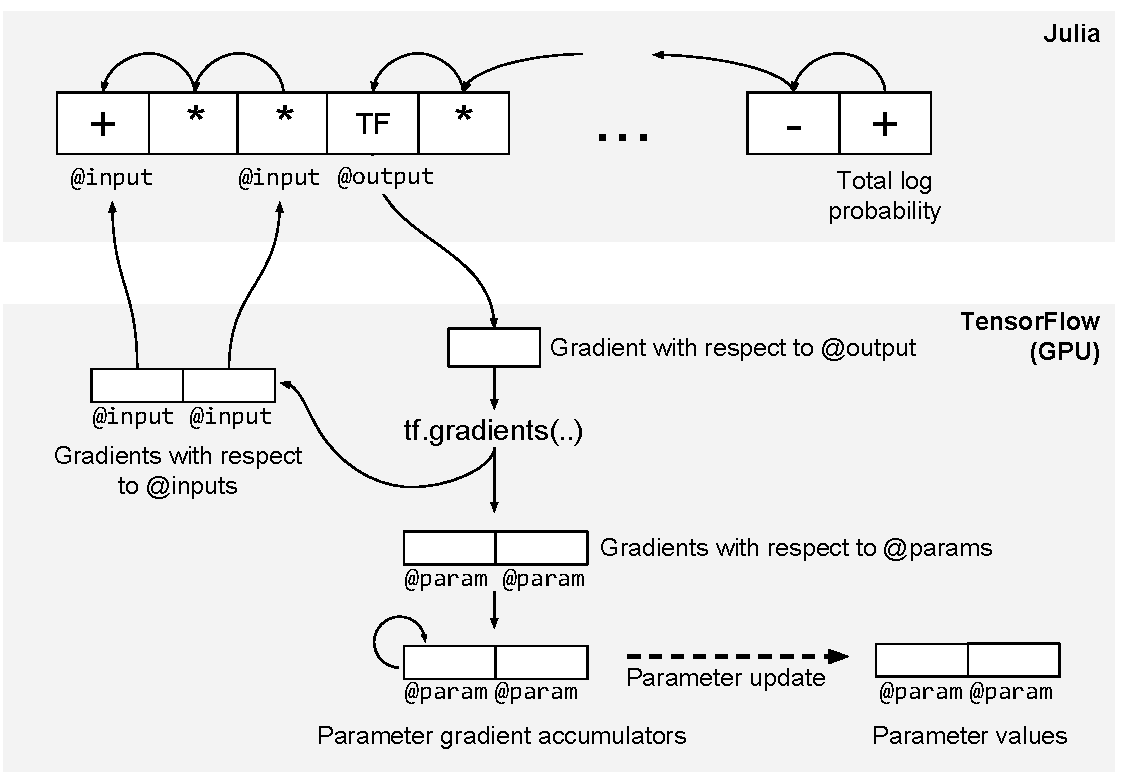
\includegraphics[width=0.7\textwidth]{images/tf-integration-schematic.pdf}
    \caption{
Reverse-mode AD in GenLite interoperates with `GenLite TensorFlow functions', which are blocks of functional TensorFlow (TF) code with inputs (corresponding to TF placeholders), trainable parameters (corresponding to TF variables), and an output, that are invoked by GenLite generative functions.
Each invocation of a TF function produces a single element on GenLite's reverse-mode AD tape.
During the backward pass (solid lines), we receive the gradient with respect to the output (\texttt{@output}) of the TF function; TF is used to compute the gradients with respect to inputs (\texttt{@input}) and parameters (\texttt{@params}).
The gradients with respect to the parameters are accumulated across multiple backward passes, until an parameter update is performed.
A parameter update (dashed line) changes the parameter values using the accumulated gradient (in addition to state of the update operation itself), and resets the gradient accumulators to zero.
Parameter updates are TF computations that are defined by the user separately from the TF function itself.
}
    \label{fig:tf-integration-schematic}
\end{figure}

\begin{figure}[t]
\begin{minipage}[t]{0.5\textwidth}
\begin{lstlisting}
using Cairo, ImageMagick, ImageFiltering
..

function render(glyph::Glyph)
  canvas = CairoRGBSurface(width, height)
  cc = CairoContext(canvas)
  Cairo.save(cc)

  # set background color to white
  Cairo.set_source_rgb(cc, 1.0, 1.0, 1.0)
  Cairo.rectangle(cc, 0.0, 0.0, width, height)
  Cairo.fill(cc)
  Cairo.restore(cc)
  Cairo.save(cc)

  # write the letter
  fontface = "Sans $(glyph.fontsize)"
  Cairo.set_font_face(cc, fontface)
  Cairo.text(cc, glyph.x, glyph.y, glyph.letter,
             angle=glyph.angle)

  return convert_to_png_blob(canvas)
end
\end{lstlisting}
\end{minipage}%
\begin{minipage}[t]{0.5\textwidth}
\begin{lstlisting}
model = @gen function()
  # prior
  x = width * @rand(uniform_cont(0, 1), <@\addr{"x"}@>)
  y = height * @rand(uniform_cont(0, 1), <@\addr{"y"}@>)
  size = @rand(uniform_cont(0, 1), <@\addr{"size"}@>)
  letter_id = @rand(uniform_disc(1, 3), <@\addr{"letter"}@>)
  letter = ["A", "B", "C"][letter_id]
  angle = 45 * @rand(uniform_cont(-1, 1), <@\addr{"angle"}@>)
  fontsize = scale_size(min_size, max_size, size)
  glyph = Glyph(x, y, angle, fontsize, letter)

  # render to png bytes
  image_png = render(glyph)

  # add Gaussian blur
  blur_width = 3
  blurred_png = imfilter(image_png,
                  Kernel.gaussian(blur_width))

  # add noise
  matrix = convert(Matrix{Float64}, blurred_png)
  @rand(speckle_noise(matrix, 0.1), <@\addr{"image"}@>)
end
\end{lstlisting}
\end{minipage}
\caption{Generative function for a generative model of blurry images that contain a single letter at a random location, rotation, and size. Addresses of random choices are shown in green.}
\label{fig:model-code-figure}
\end{figure}

\begin{figure}[t]
\begin{minipage}[t]{0.5\textwidth}
\begin{lstlisting}
using GenLiteTF
using TensorFlow
tf = TensorFlow

num_input = width * height
num_output = 11

function conv2d(x, W)
  tf.nn.conv2d(x, W, [1, 1, 1, 1], "SAME")
end

function max_pool_2x2(x)
  tf.nn.max_pool(x, [1, 2, 2, 1], [1, 2, 2, 1], "SAME")
end

function initial_weight(shape)
  randn(Float32, shape...) * 0.001f0
end

function initial_bias(shape)
  fill(0.1f0, shape...)
end

network = @tf_function begin

  # input image (N, 56 * 56)
  @input image_flat Float32 [-1, num_input]
  image = tf.reshape(image_flat, [-1, width, height, 1])

  # convolution + max-pooling (N, 28, 28, 32)
  @param W_conv1 initial_weight([5, 5, 1, 32])
  @param b_conv1 initial_bias([32])
  h_conv1 = tf.nn.relu(conv2d(image, W_conv1) + b_conv1)
  h_pool1 = max_pool_2x2(h_conv1)

  # convolution + max-pooling (N, 14, 14, 32)
  @param W_conv2 initial_weight([5, 5, 32, 32])
  @param b_conv2 initial_bias([32])
  h_conv2 = tf.nn.relu(conv2d(h_pool1, W_conv2) + b_conv2)
  h_pool2 = max_pool_2x2(h_conv2)
  h_pool2_flat = tf.reshape(h_pool2, [-1, 14 * 14 * 32])

  # convolution + max-pooling (N, 7, 7, 64)
  @param W_conv3 initial_weight([5, 5, 32, 64])
  @param b_conv3 initial_bias([64])
  h_conv3 = tf.nn.relu(conv2d(h_pool2, W_conv3) + b_conv3)
  h_pool3 = max_pool_2x2(h_conv3)
  h_pool3_flat = tf.reshape(h_pool3, [-1, 7 * 7 * 64])

  # fully connected layer (N, 1024)
  @param W_fc1 initial_weight([7 * 7 * 64, 1024])
  @param b_fc1 initial_bias([1024])
  h_fc1 = tf.nn.relu(h_pool3_flat * W_fc1 + b_fc1)

  # output layer (N, 11)
  @param W_fc2 initial_weight([1024, num_output])
  @param b_fc2 initial_bias([num_output])
  @output Float32 (tf.matmul(h_fc1, W_fc2) + b_fc2)
end

\end{lstlisting}
\end{minipage}%
\hfill
\begin{minipage}[t]{0.4\textwidth}
\begin{lstlisting}
predict = @gen function (outputs)

  # predict the x-coordinate
  x_mu = outputs[1]
  x_std = exp(outputs[2])
  @rand(normal(x_mu, x_std), <@\addr{"x"}@>)

  # predict the y-coordinate
  y_mu = outputs[3]
  y_std = exp(outputs[4])
  @rand(normal(y_mu, y_std), <@\addr{"y"}@>)

  # predict the rotation
  r_mu = exp(outputs[5])
  r_std = exp(outputs[6])
  @rand(normal(r_mu, r_std), <@\addr{"angle"}@>)

  # predict the size 
  size_alpha = exp(outputs[7])
  size_beta = exp(outputs[8])
  @rand(Gen.beta(size_alpha, size_beta), <@\addr{"size"}@>)
  
  # predict the identity of the letter
  log_letter_dist = outputs[9:end]
  letter_dist = exp.(log_letter_dist)
  letter_dist = letter_dist / sum(letter_dist)
  @rand(categorical(letter_dist), <@\addr{"letter"}@>)
end

proposal = @gen function ()

  # get image from input trace
  image = zeros(1, num_input)
  image[1,:] = @read(<@\addr{"image"}@>)[:]

  # run inference network
  outputs = @tf_call(network(image))

  # make prediction given inference network outputs
  @splice(predict(outputs[1,:]))
end

proposal_batch = @gen function (batch_size)

  # get images from input trace
  images = zeros(Float32, batch_size, num_input)
  for i=1:batch_size
    images[i,:] = @read((<@\addr{"\$i"}@>, <@\addr{"image"}@>))[:]
  end

  # run inference network in batch
  outputs = @tf_call(network(images))
  
  # make prediction for each image
  for i=1:batch_size
    @call(predict(outputs[i,:]), <@\addr{"\$i"}@>)
  end
end
\end{lstlisting}
\end{minipage}
\caption{
A GenLite TensorFlow (TF) function (\texttt{network}) that is invoked by a generative function (\texttt{proposal}) that implements a data-driven proposal for the model of Figure~\ref{fig:model-code-figure}.
GenLite TF functions are identified by a \texttt{@tf\_function} keyword.
The user declares inputs (\texttt{@input}, corresponding to TF placeholders), parameters (\texttt{@param}, corresponding to TF variables) and an output tensor (\texttt{@output}).
The rest of the code inside the \texttt{@tf\_function} block is regular TensorFlow code, using the TensorFlow.jl Julia wrapper \cite{?} around the TensorFlow C API.
The proposal reads the image from an input trace, runs the network, and then uses its output to parametrize distributions on the latent variables in the model.
To scalably train the network on GPU hardware, we also implement a batched variant of the proposal program, which reads from and writes to vector-shaped traces.
The batched and unbatched variants of the reuse both the TensorFlow and probabilistic prediction code.
}
\label{fig:proposal-code-figure}
\end{figure}


%x = width * @rand(uniform_cont(0, 1), <@\addr{"x"}@>)

\begin{figure}[t]
\begin{subfigure}[b]{0.6\textwidth}
\begin{lstlisting}
grads_and_vars = []
zero_grad_ops = []
for (param_name) in <@\infr{get\_param\_names}@>(network)
  grad = tf.negative(<@\infr{get\_param\_grad}@>(network, param_name))
  var = <@\infr{get\_param\_var}@>(network, param_name)
  push!(grads_and_vars, (grad, var))
  push!(zero_grad_ops, <@\infr{get\_zero\_grad\_op}@>(network, param_name))
end
optimizer = tf.train.AdamOptimizer(1e-4)
network_update = tf.group(
  tf.train.apply_gradients(optimizer, grads_and_vars),
  zero_grad_ops...)
\end{lstlisting}
\caption{Defining the update to the TensorFlow parameters}
\end{subfigure}%
\begin{subfigure}[b]{0.4\textwidth}
\begin{lstlisting}
num_train = 100000
traces = Vector{Trace}(num_train)
for i=1:num_train
  (traces[i], _, _) = <@\infr{simulate}@>(model, ())
end
\end{lstlisting}
\caption{Simulating training data from the model}
\end{subfigure}
\begin{subfigure}[b]{\textwidth}
\begin{lstlisting}
tf.run(get_tf_session(), tf.global_variables_initializer())
batch_size = 100
for iter=1:num_iter
  batch_idx = randperm(num_train)[1:batch_size]
  traces = all_traces[batch_idx]
  vector_trace = <@\infr{vectorize}@>(traces)
  (total_score, _) = <@\infr{backprop}@>(proposal_batch, (batch_size,), vector_trace, vector_trace)
  tf.run(get_tf_session(), network_update)
  score = total_score / batch_size
end
\end{lstlisting}
\caption{Training the proposal on simulated data}
\end{subfigure}
\caption{
Julia code for training the data-driven proposal distribution of Figure~\ref{fig:proposal-code-figure} to propose the latent variables of the generative model (\texttt{model}) of Figure~\ref{fig:model-code-figure} given an observed image.
In (a), we define an TensorFlow (TF) operation (\texttt{network\_update}) that will be used to update the parameters of the TF function \texttt{network} (defined in Figure~\ref{fig:proposal-code-figure}.
We define the operation in terms of the parameter value variables and parameter gradient accumulator variables that are accessible with GenLite API functions \texttt{get\_param\_var} and \texttt{get\_param\_grad}, respectively.
The update applies an ADAM update to all of the parameters and then zeros-out the gradient accumulators.
Next, in (b), we generate training data by sampling traces from the model.
These traces contain both the observed image (at address \texttt{"image"}) and all of the latent variables (\texttt{"x"}, \texttt{"y"}, ..).
Finally, in (c), we perform training using batches.
We group a set of traces of \texttt{model} into a vector-shaped trace using \texttt{vectorize}.
We then run \texttt{backprop} on the generative function \texttt{proposal\_batch}, where we use \texttt{vector\_trace} as both the input trace (from which the image is read) and the output trace (which contains the ground truth latent variables for the corresponding image).
GenLite API functions are shown in purple.
}
\label{fig:training-code-figure}
\end{figure}

\begin{figure}[t]
\begin{minipage}[t]{0.55\textwidth}
\begin{lstlisting}
function importance_sample(input_image, num_samples)
  observations = Trace()
  observations[<@\addr{"image"}@>] = input_image

  # obtain importance samples and their weights
  traces = Vector{Trace}(num_samples)
  log_weights = Vector{Float64}(num_samples)
  for i=1:num_samples
    (traces[i], _, log_weights[i], _) = <@\infr{importance2}@>(
      model, (), proposal, (), observations)
  end

  # return trace with probability proportional to its weight
  probs = exp.(log_weights - logsumexp(log_weights))
  idx = rand(categorical, (probs,))
  return traces[idx]
end
\end{lstlisting}
\end{minipage}
\caption{
Performing inference in the generative model of Figure~\ref{fig:model-code-figure} using a combination of deep learning and model-based Monte Carlo.
Having trained the proposal distribution (\texttt{proposal}) we use it as an importance distribution in a sampling-importance-resampling algorithm.
The GenLite API function \infr{\texttt{importance2}} samples from an importance distribution by simulating from a generative function, and then treats the resulting trace as a proposed trace for the model.
}
\label{fig:inference-code-figure}
\end{figure}



\section{Examples}

\subsection{Character recognition}
This section illustrates the technique using a computer vision application.
Figure~\ref{fig:model-code-figure} shows a generative model for blurry images of letters, expressed as a generative function in GenLite.
The model first samples the location, orientiation, size, and identity of the letter from a prior distribution, then renders the image using a graphics library, adds Gaussian blur to the image, and finally adds independent pixel-wise `speckle' noise to the image.
Figure~\ref{fig:proposal-code-figure} shows a data-driven proposal for the latent variables of the generative model given the observed image, also expressed as a generative function.
This generative function invokes a deep convolutional neural network implemented in TensorFlow.
Next, Figure~\ref{fig:training-code-figure} shows the code for training the proposal on data generated from the generative model.
Figure~\ref{fig:inference-code-figure} shows the implementation of an sampling-importance-resampling algorithm that uses the trained proposal.
Finally, Figure~\ref{fig:example-results} shows an observed image, as well as renderings of the latent variables produced from importance sampling using the trained proposal.

\begin{figure}[h]
\centering
    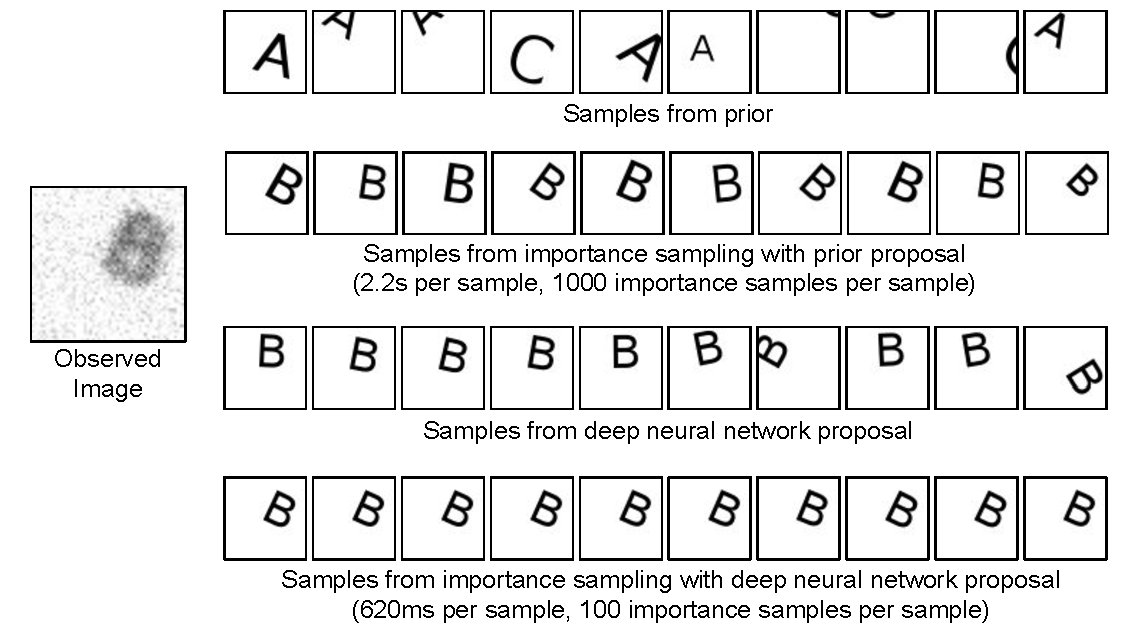
\includegraphics[width=1.0\textwidth]{images/deep-neural-network-is.pdf}
    \caption{
Results of inference in the generative model of Figure~\ref{fig:model-code-figure} using a combination of deep learning and model-based Monte Carlo.
On the left is the observed image, followed by a set of 10 of latent images sampled from the trained deep neural network proposal (\texttt{proposal} in Figure~\ref{fig:proposal-code-figure}), and a set of 10 latent images sampled using importance sampling, with the trained deep neural network proposal as the importance distribution.
The deep neural network was trained on traces and images jointly sampled from the generative model, using ADAM with 170,000 iterations, each with batch size 100 (total time 5hrs on Tesla K80 GPU).
The deep neural network proposal is uncertain about the location and orientiation of the letter.
Augmenting the neural network with model-based importance sampling gives more accurate inferences.
}
    \label{fig:example-results}
\end{figure}

\begin{figure}[t]
\begin{minipage}[t]{0.5\textwidth}
\begin{lstlisting}
using Cairo, ImageMagick, ImageFiltering
..

function render(glyph::Glyph)
  canvas = CairoRGBSurface(width, height)
  cc = CairoContext(canvas)
  Cairo.save(cc)

  # set background color to white
  Cairo.set_source_rgb(cc, 1.0, 1.0, 1.0)
  Cairo.rectangle(cc, 0.0, 0.0, width, height)
  Cairo.fill(cc)
  Cairo.restore(cc)
  Cairo.save(cc)

  # write the letter
  fontface = "Sans $(glyph.fontsize)"
  Cairo.set_font_face(cc, fontface)
  Cairo.text(cc, glyph.x, glyph.y, glyph.letter,
             angle=glyph.angle)

  return convert_to_png_blob(canvas)
end
\end{lstlisting}
\end{minipage}%
\begin{minipage}[t]{0.5\textwidth}
\begin{lstlisting}
model = @gen function()
  # prior
  x = width * @rand(uniform_cont(0, 1), <@\addr{"x"}@>)
  y = height * @rand(uniform_cont(0, 1), <@\addr{"y"}@>)
  size = @rand(uniform_cont(0, 1), <@\addr{"size"}@>)
  letter_id = @rand(uniform_disc(1, 3), <@\addr{"letter"}@>)
  letter = ["A", "B", "C"][letter_id]
  angle = 45 * @rand(uniform_cont(-1, 1), <@\addr{"angle"}@>)
  fontsize = scale_size(min_size, max_size, size)
  glyph = Glyph(x, y, angle, fontsize, letter)

  # render to png bytes
  image_png = render(glyph)

  # add Gaussian blur
  blur_width = 3
  blurred_png = imfilter(image_png,
                  Kernel.gaussian(blur_width))

  # add noise
  matrix = convert(Matrix{Float64}, blurred_png)
  @rand(speckle_noise(matrix, 0.1), <@\addr{"image"}@>)
end
\end{lstlisting}
\end{minipage}
\caption{Generative function for a generative model of blurry images that contain a single letter at a random location, rotation, and size. Addresses of random choices are shown in green.}
\label{fig:model-code-figure}
\end{figure}

\begin{figure}[t]
\begin{minipage}[t]{0.5\textwidth}
\begin{lstlisting}
using GenLiteTF
using TensorFlow
tf = TensorFlow

num_input = width * height
num_output = 11

function conv2d(x, W)
  tf.nn.conv2d(x, W, [1, 1, 1, 1], "SAME")
end

function max_pool_2x2(x)
  tf.nn.max_pool(x, [1, 2, 2, 1], [1, 2, 2, 1], "SAME")
end

function initial_weight(shape)
  randn(Float32, shape...) * 0.001f0
end

function initial_bias(shape)
  fill(0.1f0, shape...)
end

network = @tf_function begin

  # input image (N, 56 * 56)
  @input image_flat Float32 [-1, num_input]
  image = tf.reshape(image_flat, [-1, width, height, 1])

  # convolution + max-pooling (N, 28, 28, 32)
  @param W_conv1 initial_weight([5, 5, 1, 32])
  @param b_conv1 initial_bias([32])
  h_conv1 = tf.nn.relu(conv2d(image, W_conv1) + b_conv1)
  h_pool1 = max_pool_2x2(h_conv1)

  # convolution + max-pooling (N, 14, 14, 32)
  @param W_conv2 initial_weight([5, 5, 32, 32])
  @param b_conv2 initial_bias([32])
  h_conv2 = tf.nn.relu(conv2d(h_pool1, W_conv2) + b_conv2)
  h_pool2 = max_pool_2x2(h_conv2)
  h_pool2_flat = tf.reshape(h_pool2, [-1, 14 * 14 * 32])

  # convolution + max-pooling (N, 7, 7, 64)
  @param W_conv3 initial_weight([5, 5, 32, 64])
  @param b_conv3 initial_bias([64])
  h_conv3 = tf.nn.relu(conv2d(h_pool2, W_conv3) + b_conv3)
  h_pool3 = max_pool_2x2(h_conv3)
  h_pool3_flat = tf.reshape(h_pool3, [-1, 7 * 7 * 64])

  # fully connected layer (N, 1024)
  @param W_fc1 initial_weight([7 * 7 * 64, 1024])
  @param b_fc1 initial_bias([1024])
  h_fc1 = tf.nn.relu(h_pool3_flat * W_fc1 + b_fc1)

  # output layer (N, 11)
  @param W_fc2 initial_weight([1024, num_output])
  @param b_fc2 initial_bias([num_output])
  @output Float32 (tf.matmul(h_fc1, W_fc2) + b_fc2)
end

\end{lstlisting}
\end{minipage}%
\hfill
\begin{minipage}[t]{0.4\textwidth}
\begin{lstlisting}
predict = @gen function (outputs)

  # predict the x-coordinate
  x_mu = outputs[1]
  x_std = exp(outputs[2])
  @rand(normal(x_mu, x_std), <@\addr{"x"}@>)

  # predict the y-coordinate
  y_mu = outputs[3]
  y_std = exp(outputs[4])
  @rand(normal(y_mu, y_std), <@\addr{"y"}@>)

  # predict the rotation
  r_mu = exp(outputs[5])
  r_std = exp(outputs[6])
  @rand(normal(r_mu, r_std), <@\addr{"angle"}@>)

  # predict the size 
  size_alpha = exp(outputs[7])
  size_beta = exp(outputs[8])
  @rand(Gen.beta(size_alpha, size_beta), <@\addr{"size"}@>)
  
  # predict the identity of the letter
  log_letter_dist = outputs[9:end]
  letter_dist = exp.(log_letter_dist)
  letter_dist = letter_dist / sum(letter_dist)
  @rand(categorical(letter_dist), <@\addr{"letter"}@>)
end

proposal = @gen function ()

  # get image from input trace
  image = zeros(1, num_input)
  image[1,:] = @read(<@\addr{"image"}@>)[:]

  # run inference network
  outputs = @tf_call(network(image))

  # make prediction given inference network outputs
  @splice(predict(outputs[1,:]))
end

proposal_batch = @gen function (batch_size)

  # get images from input trace
  images = zeros(Float32, batch_size, num_input)
  for i=1:batch_size
    images[i,:] = @read((<@\addr{"\$i"}@>, <@\addr{"image"}@>))[:]
  end

  # run inference network in batch
  outputs = @tf_call(network(images))
  
  # make prediction for each image
  for i=1:batch_size
    @call(predict(outputs[i,:]), <@\addr{"\$i"}@>)
  end
end
\end{lstlisting}
\end{minipage}
\caption{
A GenLite TensorFlow (TF) function (\texttt{network}) that is invoked by a generative function (\texttt{proposal}) that implements a data-driven proposal for the model of Figure~\ref{fig:model-code-figure}.
GenLite TF functions are identified by a \texttt{@tf\_function} keyword.
The user declares inputs (\texttt{@input}, corresponding to TF placeholders), parameters (\texttt{@param}, corresponding to TF variables) and an output tensor (\texttt{@output}).
The rest of the code inside the \texttt{@tf\_function} block is regular TensorFlow code, using the TensorFlow.jl Julia wrapper \cite{?} around the TensorFlow C API.
The proposal reads the image from an input trace, runs the network, and then uses its output to parametrize distributions on the latent variables in the model.
To scalably train the network on GPU hardware, we also implement a batched variant of the proposal program, which reads from and writes to vector-shaped traces.
The batched and unbatched variants of the reuse both the TensorFlow and probabilistic prediction code.
}
\label{fig:proposal-code-figure}
\end{figure}


%x = width * @rand(uniform_cont(0, 1), <@\addr{"x"}@>)

\begin{figure}[t]
\begin{subfigure}[b]{0.6\textwidth}
\begin{lstlisting}
grads_and_vars = []
zero_grad_ops = []
for (param_name) in <@\infr{get\_param\_names}@>(network)
  grad = tf.negative(<@\infr{get\_param\_grad}@>(network, param_name))
  var = <@\infr{get\_param\_var}@>(network, param_name)
  push!(grads_and_vars, (grad, var))
  push!(zero_grad_ops, <@\infr{get\_zero\_grad\_op}@>(network, param_name))
end
optimizer = tf.train.AdamOptimizer(1e-4)
network_update = tf.group(
  tf.train.apply_gradients(optimizer, grads_and_vars),
  zero_grad_ops...)
\end{lstlisting}
\caption{Defining the update to the TensorFlow parameters}
\end{subfigure}%
\begin{subfigure}[b]{0.4\textwidth}
\begin{lstlisting}
num_train = 100000
traces = Vector{Trace}(num_train)
for i=1:num_train
  (traces[i], _, _) = <@\infr{simulate}@>(model, ())
end
\end{lstlisting}
\caption{Simulating training data from the model}
\end{subfigure}
\begin{subfigure}[b]{\textwidth}
\begin{lstlisting}
tf.run(get_tf_session(), tf.global_variables_initializer())
batch_size = 100
for iter=1:num_iter
  batch_idx = randperm(num_train)[1:batch_size]
  traces = all_traces[batch_idx]
  vector_trace = <@\infr{vectorize}@>(traces)
  (total_score, _) = <@\infr{backprop}@>(proposal_batch, (batch_size,), vector_trace, vector_trace)
  tf.run(get_tf_session(), network_update)
  score = total_score / batch_size
end
\end{lstlisting}
\caption{Training the proposal on simulated data}
\end{subfigure}
\caption{
Julia code for training the data-driven proposal distribution of Figure~\ref{fig:proposal-code-figure} to propose the latent variables of the generative model (\texttt{model}) of Figure~\ref{fig:model-code-figure} given an observed image.
In (a), we define an TensorFlow (TF) operation (\texttt{network\_update}) that will be used to update the parameters of the TF function \texttt{network} (defined in Figure~\ref{fig:proposal-code-figure}.
We define the operation in terms of the parameter value variables and parameter gradient accumulator variables that are accessible with GenLite API functions \texttt{get\_param\_var} and \texttt{get\_param\_grad}, respectively.
The update applies an ADAM update to all of the parameters and then zeros-out the gradient accumulators.
Next, in (b), we generate training data by sampling traces from the model.
These traces contain both the observed image (at address \texttt{"image"}) and all of the latent variables (\texttt{"x"}, \texttt{"y"}, ..).
Finally, in (c), we perform training using batches.
We group a set of traces of \texttt{model} into a vector-shaped trace using \texttt{vectorize}.
We then run \texttt{backprop} on the generative function \texttt{proposal\_batch}, where we use \texttt{vector\_trace} as both the input trace (from which the image is read) and the output trace (which contains the ground truth latent variables for the corresponding image).
GenLite API functions are shown in purple.
}
\label{fig:training-code-figure}
\end{figure}

\begin{figure}[t]
\begin{minipage}[t]{0.55\textwidth}
\begin{lstlisting}
function importance_sample(input_image, num_samples)
  observations = Trace()
  observations[<@\addr{"image"}@>] = input_image

  # obtain importance samples and their weights
  traces = Vector{Trace}(num_samples)
  log_weights = Vector{Float64}(num_samples)
  for i=1:num_samples
    (traces[i], _, log_weights[i], _) = <@\infr{importance2}@>(
      model, (), proposal, (), observations)
  end

  # return trace with probability proportional to its weight
  probs = exp.(log_weights - logsumexp(log_weights))
  idx = rand(categorical, (probs,))
  return traces[idx]
end
\end{lstlisting}
\end{minipage}
\caption{
Performing inference in the generative model of Figure~\ref{fig:model-code-figure} using a combination of deep learning and model-based Monte Carlo.
Having trained the proposal distribution (\texttt{proposal}) we use it as an importance distribution in a sampling-importance-resampling algorithm.
The GenLite API function \infr{\texttt{importance2}} samples from an importance distribution by simulating from a generative function, and then treats the resulting trace as a proposed trace for the model.
}
\label{fig:inference-code-figure}
\end{figure}


\subsection{Inferring human body pose from depth image}

\section{Related Work}
\begin{itemize}
\item Guide programs in Pyro
\item Using probabilisic programs as proposals \cite{cusumano2018using}
\item Edward \cite{tran2016edward}
\item Stuart Russell work on block neural proposals \cite{wang2017neural}
\item Univeral compiled inference in probabilistic programs \cite{le2016inference}
\item Stochastic inverses \cite{stuhlmuller2013learning}
\item Wake sleep, Helmholtz machines, VAE
\item Other work on data-driven proposals (e.g. \cite{tu2002image}).
\end{itemize}

\section{Discussion}


\subsubsection*{Acknowledgments}
This research was supported by DARPA (PPAML program, contract number FA8750-14-2-0004), IARPA (under research contract 2015-15061000003), the Office of Naval Research (under research contract N000141310333), the Army Research Office (under agreement number W911NF-13-1-0212), and gifts from Analog Devices and Google.
This research was conducted with Government support under and awarded by DoD, Air Force Office of Scientific Research, National Defense Science and Engineering Graduate (NDSEG) Fellowship, 32 CFR 168a.

\bibliographystyle{unsrtnat}
\bibliography{references}

\end{document}
